\chapter{Formas bilineales y cuadráticas}

En este capítulo  se dará una breve introducción al tema enfocada a
mostrar  aplicaciones de lo diagonalización de las matrices de las formas bilineales y cuadráticas  en el estudio  de secciones cónicas y superficies cuádricas. . 




\section{Formas bilineales y cuadráticas}

La ecuación general de una cónica está dada por una ecuación de segundo grado de la forma
\begin{equation}
a_{11}x_1^{2}+a_{12}x_1x_2+a_{22}x_2^{2}+ a_1 x_1 + a_2 x_2 + a = 0, \label{fcuadratica0}
\end{equation}
donde $a_{ij}$, $a_i$ ($i,j=1,2$) y $a$ son números reales  y al menos uno de los números $a_{ij}$ no es cero.
La parte principal es:



\begin{equation}
a_{11}x^{2}+a_{12}xy+a_{22}y^{2}
\end{equation}
\noindent
y puede escribirse

\begin{equation}
P(x,y)=a_{11}x^{2}+a_{12}xy+a_{22}y^{2}=(x, y) ~A \left(\begin{array}{c} x \\  y 
 \end{array}\right), \label{fcuadratica01}
\end{equation}


\bigskip
\noindent
donde $A$ es la matriz simétrica,
\begin{equation}
A= \left(\begin{array}{cc} a_{11} & a_{12}/2  \\a_{12}/2 & a_{22}
\end{array}
 \right). \label{fcmatriz}
\end{equation}

\bigskip



Y su generalización a $\mathbb{R}^{n}$, dado $\vec{x}=(x_1, x_2, x_3, \cdots, x_n) \in$ $\mathbb{R}^{n}$, es 



\begin{equation}
\label{fcuadratica01Rn}
P(\vec{x})=(x_1, x_2, x_3, \cdots, x_n)A \left(\begin{array}{c}  x_{1} \\  x_{2}  
\\  x_3 \\ \cdots \\  x_{n} 
\end{array}\right)
\end{equation}

\bigskip

\bigskip

\noindent
donde  $A$ es una matriz  simétrica $\in$ $\mathbb{R}^{n \times n}.$

\noindent
Análogamente al caso $n=2$, para $n=3$ se obtienen superficies de segundo grado.

\bigskip

Los dos ejemplos anteriores corresponden a   \textit{formas cuadráticas} (en $\mathbb{R}^{2}$ y en  $\mathbb{R}^{n}$), y son casos particulares de \textit{formas bilineales}, las que se definen a continuación.

\bigskip

\begin{definition}\textbf{Forma bilineal}\index{Forma bilineal}


Sea $V$ un espacio vectorial sobre $\mathbb{R}$ o $\mathbb{C}$. Una aplicación $\mathbf{A}:  V \times V\rightarrow \mathbb{R}$ (o $\mathbb{C}$) se dice que es una \textit{forma bilineal} sí y solo sí satisface:

\bigskip

\begin{enumerate}



\item  

$\mathbf{A}(\vec{x}+\vec{z},\vec{y}   )=\mathbf{A}(\vec{x},\vec{y}) + \mathbf{A}(\vec{z},\vec{y})$, $~ \forall~$  $\vec{x}$, $\vec{y}$, $\vec{z} $ $\in V$
\bigskip


\item $\mathbf{A}(\alpha\vec{x},\vec{y})=\alpha \mathbf{A} (\vec{x},\vec{y})$ $~ \forall~$$\vec{x}$, $\vec{y}$ $\in V$ y $~ \forall~$ $\alpha \in \mathbb{R} $ o $\mathbb{C}$

\bigskip


\item $\mathbf{A}(\vec{x},\vec{y} +\vec{z}  )=\mathbf{A}(\vec{x},\vec{y}) + \mathbf{A}(\vec{x},\vec{z})$, $~ \forall~$ $\vec{x}$, $\vec{y}$, $\vec{z} $ $\in V$

\bigskip


\item  $\mathbf{A}(\vec{x},\beta \vec{y})= \beta \mathbf{A}(\vec{x}, \vec{y})$ $~ \forall~$ $\vec{x}$, $\vec{y}$ y $~ \forall~$ $\beta \in \mathbb{R} $ o $\mathbb{C}$

\end{enumerate}


\end{definition}

\bigskip

\bigskip

\begin{remark}
Los productos internos reales son formas bilineales.
\end{remark}

\bigskip

\bigskip


\begin{example}
$\mathbb{E}$ un espacio  Euclídeo de dimensión finita, y $T$ una aplicación lineal de $\mathbb{E}$ en $\mathbb{E}$. Puede demostrarse que  $\mathbf{A}(\vec{x},\vec{y})=(\vec{x}, T \vec{y})$ es una forma bilineal.
\end{example}

\bigskip

\begin{example} 
Dados 

$\vec{x}=(x_1, x_2, x_3, \cdots, x_n)$ e $\vec{y}=(y_1, y_2, y_3, \cdots, y_n) \in$ $\mathbb{R}^{n}$,

$$P(\vec{x})=(x_1, x_2, x_3, \cdots, x_n)A \left(\begin{array}{c}  y_{1} \\  y_{2}  
\\  y_3 \\ \cdots \\  y_{n} 
\end{array}\right)$$

\noindent
donde  $A$ es una matriz  simétrica $\in$ $\mathbb{R}^{n \times n}$, es una forma bilineal.


\bigskip

La forma cuadrática en $\mathbb{R}^{n}$ de la Ec.(\ref{fcuadratica01Rn}) presentada antes sale de tomar para estee caso $\vec{x}=\vec{y}$.
\end{example}

\bigskip



\bigskip

\begin{remark}
\begin{itemize}
    \item 

Una forma bilineal se dice \textit{simétrica} si  $A(\vec{x},\vec{y})= A(\vec{y},\vec{x})$

\item 

Una forma bilineal se dice \textit{ antisimétrica} si  $A(\vec{x},\vec{y})= -A(\vec{y},\vec{x})$
\end{itemize}
\end{remark}

\bigskip

\begin{definition}\textbf{Matriz de una forma bilineal} \index{Matriz de una forma bilineal}

\bigskip

Sea  $\mathbf{A}$ una forma bilineal en un espacio $V$ y sea $B= \left\{\vec{e}_1,\vec{e}_2,\cdots, \vec{e}_n\right\}$ una base de $V$.


\bigskip

Si $\vec{x}=\sum^{n}_{i=1}x_i \vec{e}_i$, e $\vec{y}=\sum^{n}_{j=1}y_j \vec{e}_j$,


\begin{eqnarray*}
\mathbf{A}(\vec{x},\vec{y})&= &\mathbf{A} (\sum^{n}_{i=1} x_i \vec{e}_i, \sum^{n}_{j=1} y_j \vec{e}_j) \\
  &=&\sum^{n}_{i=1}\sum^{n}_{j=1} x_i y_j \mathbf{A}(\vec{e}_i, \vec{e}_j)
  \end{eqnarray*}


 Se define  la matriz de la forma bilineal $\mathbf{A}$ en la base $B$ como la matriz  $A \in \mathbb{R }^{n \times n }$    tal que $A_ {ij}= \mathbf{A}(\vec{e}_i,\vec{e}_j)$ para $1\leq i,j\leq n$
\end{definition}



\newpage






\begin{remark}
\begin{itemize}
    \item 
    
    Si $\mathbf{A}(\vec{x},\vec{y})= \mathbf{A}(\vec{y},\vec{x})$ (es decir $\mathbf{A}$ es una forma bilineal simétrica), entonces 
$\mathbf{A}(\vec{e}_i,\vec{e}_j) = \mathbf{A}(\vec{e}_j,\vec{e}_i)$   para cualquier base  $\left\{\vec{e}_1,\vec{e}_2,\cdots, \vec{e}_n\right\}$ de $V$, es decir la matriz de una forma bilineal $A$ simétrica en cualquier base es simétrica. 
Vale también la recíproca: si la matriz de una forma bilineal es simétrica en alguna base 
$\left\{\vec{e}_1,\vec{e}_2,\cdots, \vec{e}_n\right\}$ de $V$, entonces la forma bilineal es simétrica, pues

\bigskip


\begin{eqnarray*}
\mathbf{A}(\vec{y},\vec{x})&=& \sum^{n}_{i,j=1} \mathbf{A}(\vec{e}_i,\vec{e}_j) y_i x_j   \\
&= &\sum^{n}_{i,j=1} a_{ij} y_i x_j   \\
&=& \sum^{n}_{i,j=1} a_{ji}  x_j y_i \\
&= &\sum^{n}_{i,j=1} \mathbf{A}(\vec{e}_j,\vec{e}_i)  x_j y_i   \\
&=& \mathbf{A}(\vec{x},\vec{y})
\end{eqnarray*}

\bigskip

\item

%bolasazules{

\bigskip
Si $\mathbf{A}$ es una forma bilineal antisimétrica, $\mathbf{A}(\vec{x},\vec{y})= -\mathbf{A}(\vec{y},\vec{x})$ para cualquier base $\left\{\vec{e}_1,\vec{e}_2,\cdots, \vec{e}_n\right\}$ de $V$. La matriz satisface $a_{ij}=-a_{ji}$, de donde $a_{ii}=0$, $i=1,   \cdots , n$.

\bigskip

\item


Si $A$ es la matriz de una forma bilineal respecto a la base  $B= \left\{\vec{e}_1,\vec{e}_2,\cdots, \vec{e}_n\right\}$ y $\tilde{A}$ con respecto a la base $\tilde{B}= \left\{\vec{u}_1,\vec{u}_2,\cdots, \vec{u}_n\right\}$, entonces $A= C^{T} \tilde{A}C$, donde $C$ es la matriz de cambio de base de $B$ a $\tilde{B}$. Tienen el mismo rango $\tilde{A}$ y $ A $, ya que $det(C) \neq 0$.

\bigskip

\item
El rango de una forma bilineal es el rango que tiene la matriz de la forma bilineal en cualquier base.

\end{itemize}

\end{remark}


\bigskip



\begin{theorem}

Toda forma bilineal puede ser representada como la suma de una forma bilineal simétrica y una forma bilineal  antisimétrica.

\bigskip

\begin{proof}
Sea $\mathbf{A}$ una forma bilineal definida en $V$ y sea $\mathbf{B}:  V \times V\rightarrow K$  definida así $$\mathbf{B}(\vec{x},\vec{y})=\mathbf{A}(\vec{x},\vec{y})+\mathbf{A}(\vec{y},\vec{x})$$
y sea $\mathbf{C}:  V \times V\rightarrow K$
$$\mathbf{C}(\vec{x},\vec{y})=\mathbf{A}(\vec{x},\vec{y})-\mathbf{A}(\vec{y},\vec{x})$$


\bigskip

$$2\mathbf{A}(\vec{x},\vec{y})=\mathbf{B}(\vec{x},\vec{y})+ \mathbf{C}(\vec{x},\vec{y})$$

\vskip.3cm

$$\mathbf{A}(\vec{x},\vec{y})= \frac{\mathbf{B}(\vec{x},\vec{y})}{2}+ \frac{\mathbf{C}(\vec{x},\vec{y})}{2}$$


\noindent
donde 

$$\mathbf{B}(\vec{y},\vec{x})=\mathbf{A}(\vec{y},\vec{x})+ \mathbf{A}(\vec{x},\vec{y})=\mathbf{B}(\vec{x},\vec{y})$$


$$\mathbf{C}(\vec{y},\vec{x})=\mathbf{A}(\vec{y},\vec{x})- \mathbf{A}(\vec{x},\vec{y})=-\mathbf{C}(\vec{x},\vec{y})$$

\bigskip

Esto es similar a lo que ocurre con una matriz $A$, que puede expresarse, 
$$A= \frac{A+A^T}{2}+ \frac{A-A^T}{2}$$
\noindent
donde   $\frac{A+A^T}{2}$   es simétrica y $\frac{A-A^T}{2}$ antisimétrica.

\end{proof}
\end{theorem}


\begin{definition} \textbf{Forma cuadrática} \index{Forma cuadrática}

\bigskip


Dada  $\mathbf{A}$ $:  V \times V\rightarrow \mathbb{R}$  una forma bilineal,  se define una \textit{forma cuadrática }

  $\mathbf{Q} :   V\rightarrow \mathbb{R}$, $\mathbf{Q}(\vec{x})=\mathbf{A}(\vec{x},\vec{x})$.

\end{definition}

\bigskip


\begin{example}
$$\mathbf{Q}(x_1,x_2)=a_{11}x_1^{2}+a_{12}x_1x_2+a_{22}x_2^{2}$$
\end{example}



Usando la matriz $P$  definida antes, Ec.(\ref{fcuadratica01}) una forma cuadrática se escribe,






$$\mathbf{Q}(\vec{x})=(x_1, x_2, x_3, \cdots, x_n)P  (x_1, x_2, x_3, \cdots, x_n) ^{T}.$$
%\end{array}\right)$$


\bigskip

En general, toda expresión de la forma

$$\mathbf{Q}(\vec{x})=\sum^{n}_{j=1} \sum^{n}_{i \le j }  a_{ij} x_i x_j$$


\bigskip


\noindent
en un espacio vectorial define una forma cuadrática, ya que alcanza con tomar la forma bilineal 
  
\[
\mathbf{A}(\vec{x},\vec{y})= \sum^{n}_{i=1} a_{ii} x_i y_i  + \sum^{n}_{j=1} \sum^{n}_{i \le j } \frac{a_{ij}}{2} x_i y_j +  \sum^{n}_{j=1} \sum^{n}_{i  > j } \frac{a_{ij}}{2}  x_j y_i  
\]

  

    
  
con   $\vec{x}= \sum^{n}_{i=1}  x_i \vec{e}_i$ e  $\vec{y}= \sum^{n}_{j=1}  y_j \vec{e}_j$.

%\end{document}


 \bigskip


 \bigskip
 
\begin{remark}
Un ejemplo de forma bilineal   es el tensor de inercia,$I(\vec{x}, \vec{y})$ pero gran parte de su interés
radica en que $I(\omega, \omega)$ da la energía de rotacíon cuando la velocidad angular es $\omega$.
\end{remark}

 \bigskip

 
\subsection{Formas cuadráticas. Aplicación a las secciones cónicas}\index{Secciones cónicas}\index{Cuadrática}


La Ec.(\ref{fcuadratica0}) se reescribe, 

$$\mathbf{Q}(x_1,x_2)=a_{11}x_1^{2}+a_{12}x_1x_2+a_{22}x_2^{2}$$


\noindent
y también  en forma matricial,
\begin{equation}
\left(\begin{array}{cc}x_1 & x_2
\end{array}
 \right) \left(\begin{array}{cc} a_{11} & a_{12}/2  \\a_{12}/2 & a_{22}
\end{array}
 \right)  \left(\begin{array}{c} x_1 \\  x_2
\end{array}
 \right)+ \left(\begin{array}{cc}a_1 & a_2
\end{array}
 \right) \left(\begin{array}{c} x_1 \\ x_2
\end{array}
 \right) +a=0\label{fcuadraticatoda}
\end{equation}

\bigskip

\begin{equation}
\bf x ^T A \bf x + K \bf x + a =0 \label{fcuadraticamatricial}
\end{equation}
\noindent
donde 
\begin{equation}
\bf x=  \left(\begin{array}{c} x \\y
\end{array}
 \right),\qquad K=\left(\begin{array}{cc}a_1 & a_2
\end{array}
 \right)\label{fcuadraticaxyk}
\end{equation}
\index{Matriz de la forma cuadrática} 
Con esta notación, la forma cuadrática asociada a la Ec.(\ref{fcuadraticamatricial}) es $ \bf x ^T A \bf x$. La matriz simétrica $A$ se denomina \textit{matriz de la forma cuadrática } $ \bf x ^T A \bf x$. 

\bigskip

\begin{example}


En la ecuación,

\begin{equation}
3x_1^{2}+5x_1x_2-7x_2^{2}+ 2 x_1 + 7 = 0, \label{ejemplo61}
\end{equation}
la matriz de la forma cuadrática es, 

\bigskip

$\left(\begin{array}{cc}3 & 5/2 \\ 5/2 & 7
\end{array}
 \right)$.
 
 \bigskip
 
\noindent
mientras que para  la ecuación

\begin{equation}
8x_1^{2}-4x_2^{2} = 0, \label{ejemplo61}
\end{equation}
la matriz de la forma cuadrática es, 

\bigskip

$\left(\begin{array}{cc}8 & 0 \\ 0 & -4
\end{array}
 \right)$.

\end{example}

 \bigskip
 
 Para una cónica  $C$  con ecuación (\ref{fcuadraticamatricial})  es posible hacer girar los ejes de coordenadas $x_1x_2$ de modo que la ecuación de la cónica, en el sistema de coordenadas $x_1^\prime x_2^\prime$, no tenga término con producto cruzado.  
 
 \begin{itemize}
 
 \item
 Se halla una matriz $O$ que diagonaliza ortogonalmente a $A$, $A=ODO^t$. Se intercambian sus columnas en el caso que el $Det(O)\neq 1 $ para asegurar que la transformación de coordenadas sea una rotación.
 
 $$\bold x=O \bold x'$$
 
  \item
  Para obtener la ecuación en el sistema $x_1^\prime x_2^\prime$  se sustituye la ecuación anterior  en la Ec.(\ref{fcuadraticamatricial}).
 
 \begin{equation}
\bf (x^\prime) ^t O^t A O \bf x^\prime  + K O \bf x^\prime + a =0 \label{fcuadraticamatricialprima}
\end{equation}
Como $O$ diagonaliza ortogonalmente a la matriz $A$, $O^t A O =\left(\begin{array}{cc} \lambda_1 & 0 \\ 0 & \lambda_2
\end{array}
 \right)$,
 donde $\lambda_1$   y  $\lambda_2$  son los autovalores de $A$. Por lo tanto, la ecuación  (\ref{fcuadraticamatricialprima}) reescribir como
 
 \begin{equation}
\left(\begin{array}{cc}x_1^\prime & x_2^\prime
\end{array}
 \right) \left(\begin{array}{cc} \lambda_1& 0  \\ 0 & \lambda_2
\end{array}
 \right)  \left(\begin{array}{c} x_1^\prime \\x_2^\prime
\end{array}
 \right)+ \left(\begin{array}{cc}a_1 & a_2
\end{array}
 \right)
 \left(\begin{array}{cc} o_{11} & o_{12}  \\ o_{21} & o_{22}
\end{array}
 \right) 
 \left(\begin{array}{c} x_1^\prime \\x_2^\prime
\end{array}
 \right) +a=0\label{fcuadraticatoda}
\end{equation}
 o bien 
 
 $$\lambda_1(x^\prime_1)^{2}+\lambda_2(x^\prime_2)^{2}  +a_1^\prime x_1^\prime+ a_2^\prime x_2^\prime +a  =0$$

 \bigskip
 
 \noindent
 donde $a_1'=a_1o_{11}+a_2o_{21}$  y $a_2'=a_1o_{12}+a_2o_{22}$. 
 %Ahora la ecuación no tiene término de producto cruzado. 
 
  \end{itemize}
  
\begin{figure}
    \centering
    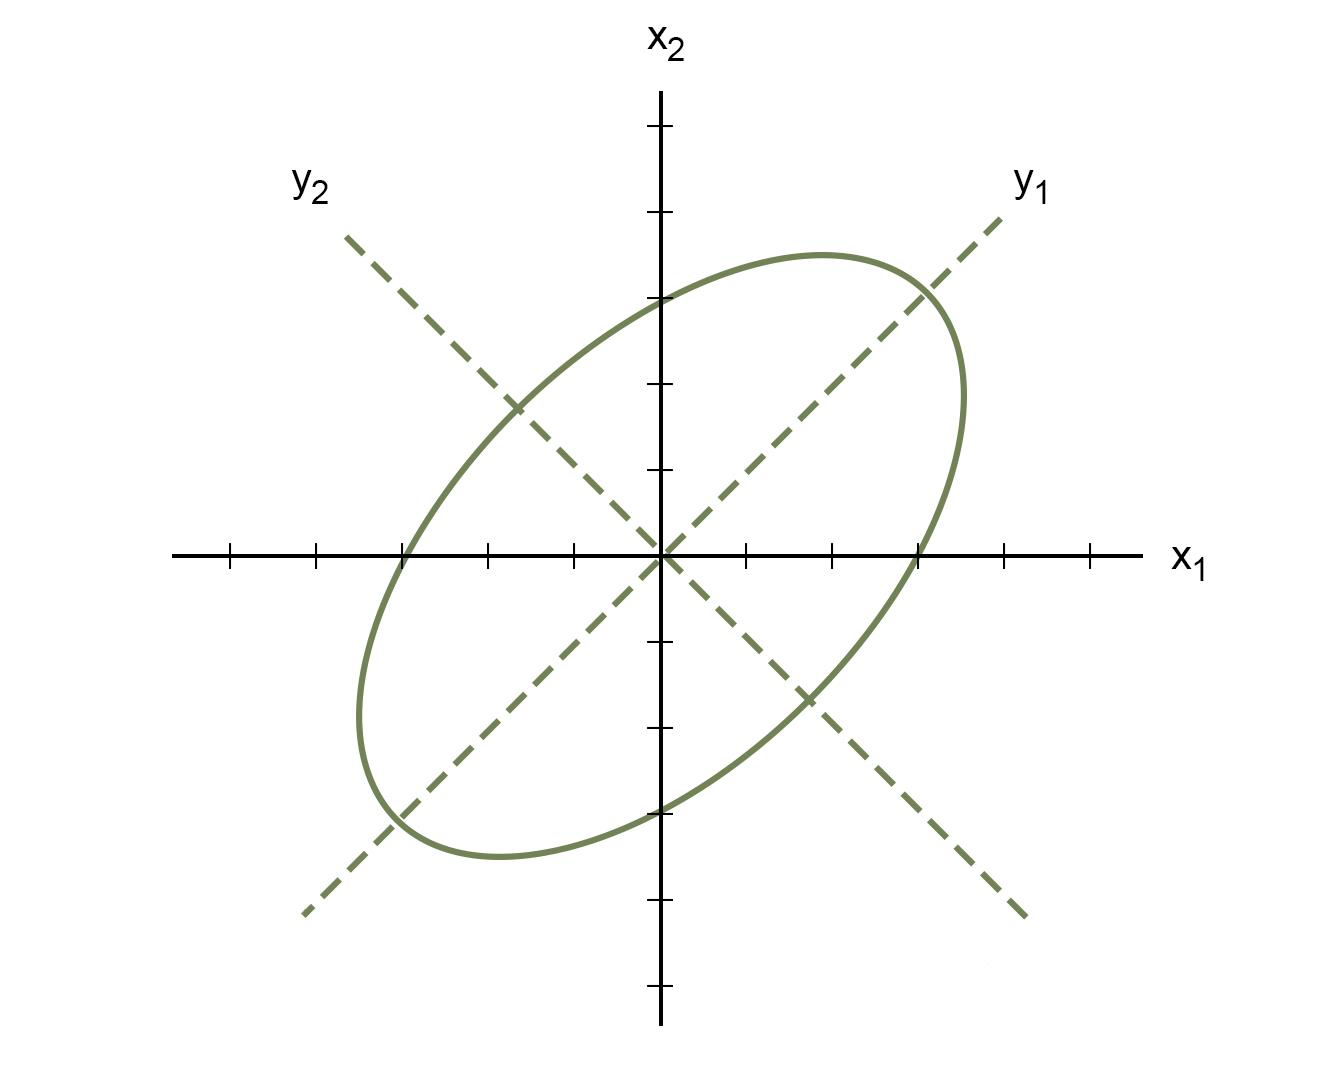
\includegraphics[width=0.75\textwidth]{Pictures/fig.29.jpg}
    \caption{Elipse}
    \label{Elipse}
\end{figure} 

  \bigskip
  
 El análisis anterior se resume en el Teorema siguiente:
 
 \bigskip
 
 \begin{corollary}\textbf{Teorema de los ejes principales para $\mathbb{R}^2$}.\index{Ejes principales $\mathbb{R}^2$}.
 
 Sea 
 \begin{equation}
a_{11}x_1^{2}+a_{12}x_1x_2+a_{22}x_2^{2}+ a_1 x_1 + a_2 x_2 + a = 0, 
\end{equation}
\noindent
la ecuación de una cónica $C$, y supongamos que 
 
 $$\bf{x} ^T A \bf{x}=a_{11}x_1^{2}+a_{12}x_1x_2+a_{22}x_2^{2}$$
 es la forma cuadrática asociada. Entonces, es posible  girar los ejes de coordenadas de modo que la ecuación para $C$ en el nuevo sistema de coordenadas $x^{\prime}y^{\prime}$ tenga la forma  
 
 $$\lambda_1x^{\prime 2}_1+\lambda_2x^{\prime 2}_2  +a_1^{\prime}x^{\prime}+ a_2^{\prime}y^{\prime} +a  =0$$
 \noindent
 donde $\lambda_1$   y  $\lambda_2$  son los autovalores de $A$. Se puede llevar a cabo la rotación por medio de la sustitución $\bold x=O \bold x^{\prime}$, donde $O$ diagonaliza a $A$ y $Det(O)=1$.
 \end{corollary}

 


\begin{figure}
    \centering
    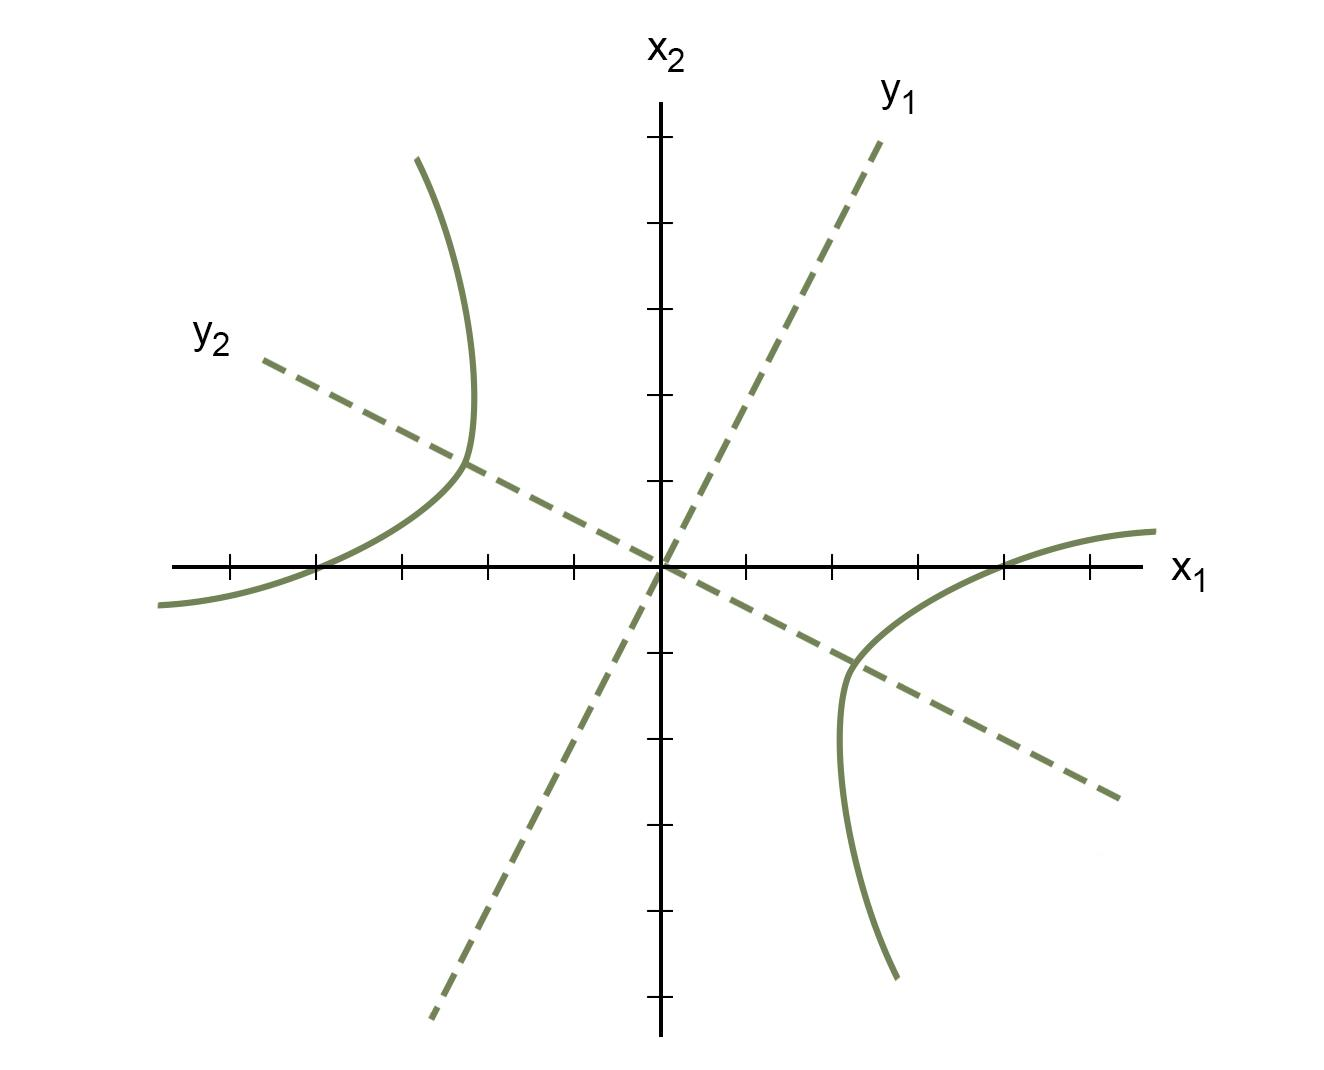
\includegraphics[width=0.75\textwidth]{Pictures/fig.30.jpg}
    \caption{Hipérbola}
    \label{Hipérbola}
\end{figure} 

Si $A$ es una matriz no diagonal, la gráfica   está girada hasta salirse de la posición estándar, como en las Figuras  \ref{Elipse} y \ref{Hipérbola}.
Encontrar los ejes principales (determinados por los vectores propios de $A$) equivale a
encontrar un nuevo sistema de coordenadas con respecto al cual la gráfica está en posición
estándar.

\bigskip

\subsection{Formas cuadráticas: aplicación a las superficies cuádricas}\index{Superficies cuádricas}
Sea
\begin{equation}
a_{11}x_1^{2}+a_{12}x_1 x_2+a_{13}x_1 x_3+a_{22}x_2^{2}+a_{23}x_2 x_3+a_{33}x_3^{2}+ a_1 x_1 + a_2 x_2+ a_3 x_3  + a = 0 \label{fcuadratica33}
\end{equation}
donde $a_{ij}$, $a_i$ ($i,j=1,3$) y $a$ son números reales  y al menos uno de los números $a_{ij}$ no es cero.
La parte principal

$$a_{11}x_1^{2}+a_{12}x_1x_2+a_{13}x_1x_3+a_{22}x_2^{2}+a_{23}x_2x_3+a_{33}x_3^{2}$$

\bigskip

 es la forma cuadrática asociada.

 \bigskip

 \bigskip
 
La Ec.(\ref{fcuadratica33}) puede escribirse en forma matricial

 \bigskip
 
\begin{equation*}
\left(\begin{array}{ccc} x & y & z 
\end{array}
 \right) \left(\begin{array}{ccc} a_{11} & a_{12}/2  & a_{13}/2  \\a_{12}/2 & a_{22} & a_{23}/2 \\a_{13}/2  & a_{23}/2 & a_{33}
\end{array}
 \right)  \left(\begin{array}{c} x \\y  \\z
\end{array}
 \right)+ \left(\begin{array}{ccc}a_1 & a_2& a_3
\end{array}
 \right) \left(\begin{array}{c} x \\y \\z 
\end{array}
 \right) +a=0\label{fcuadraticatodaR3
 }
\end{equation*}

 \bigskip
\begin{figure}
    \centering
    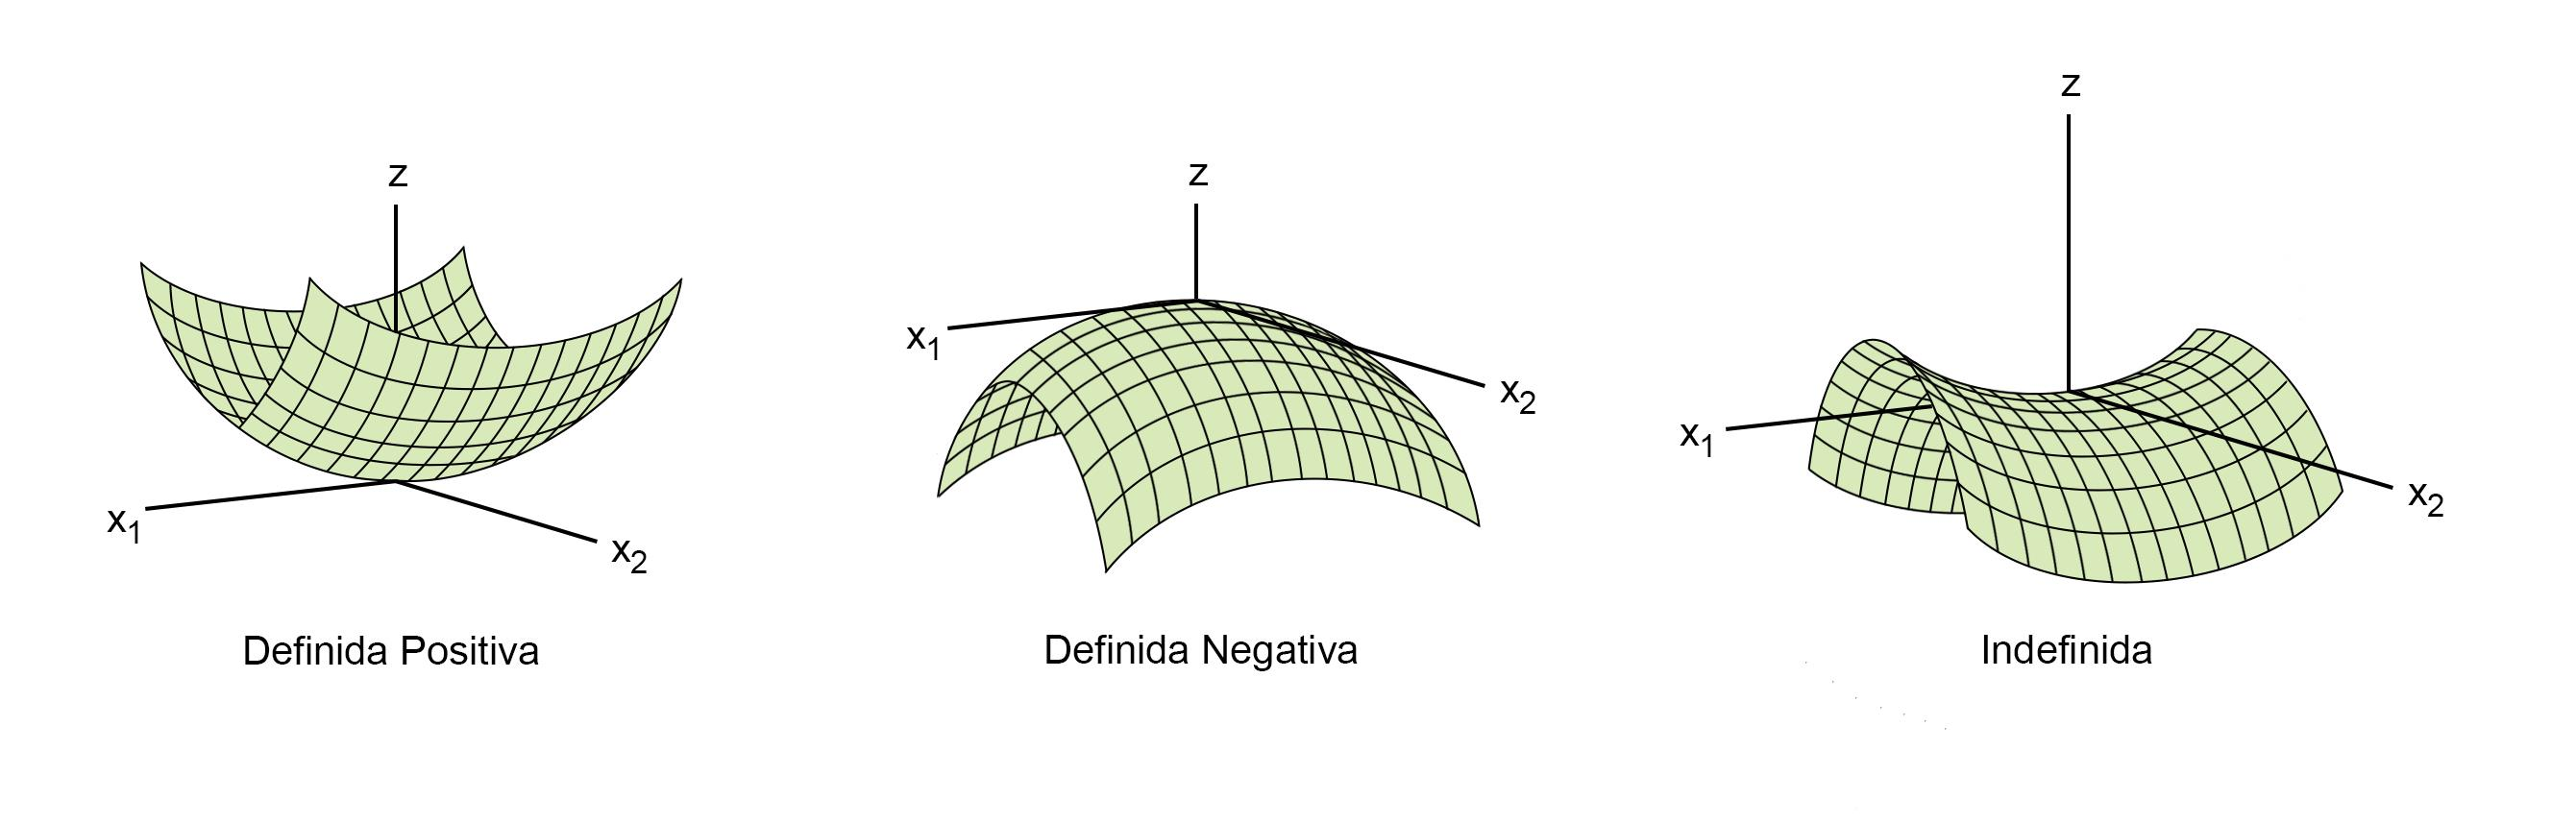
\includegraphics[width=1.1\textwidth]{Pictures/fig.31.jpg}
    \caption{Formas cuadráticas. a) Definida Positiva. b) Definida Negativa. c) Indefinida.}
    \label{FCUADRATICAS}
\end{figure} 

Se tiene el Teorema siguiente:

 \bigskip
 \begin{corollary}
     
 \textbf{Teorema de los ejes principales para $\mathbb{R}^3$}.
 
 Sea 
 \begin{equation*}
a_{11}x_1^{2}+a_{12}x_1x_2+a_{13}x_1x_3+a_{22}x_2^{2}+ 

a_{23}x_2x_3+a_{33}x_3^{2}+ a_1 x_1 + a_2 x_2+ a_3 x_3  + a = 0\label{fcuadratica3}
\end{equation*}


la ecuación de una cónica $C$, y supongamos que 
 
 $$\bf{x} ^T A \bf{x}=a_{11}x_1^{2}+a_{12}x_1x_2+a_{13}x_1x_3+a_{22}x_2^{2}+a_{23}x_2x_3+a_{33}x_3^{2}$$
 es la forma cuadrática asociada. Entonces se puede hacer girar los ejes de coordenadas de modo que la ecuación para $C$ en el nuevo sistema de coordenadas $x_1'x_2'x_3'$ tenga la forma  
 
 $$\lambda_1x^{\prime 2}_1+\lambda_2x^{\prime} 2_2+\lambda_3x^{\prime 2}_3  +a_1^{\prime}x_1^{\prime}+ a_2^{\prime}x_2^{\prime}+a_3 x_3^{\prime} +a  =0$$
 donde $\lambda_1$,   $\lambda_2$ y $\lambda_3$ son los autovalores de $A$. Como en el caso de $\mathbb{R}^2$ se puede llevar a cabo la rotación por medio de la sustitución $\bold x=O \bold x'$, donde $O$ diagonaliza a $A$ y $Det(O)=1$.
 \end{corollary}
 
 Este teorema sugiere el procedimiento para eleminar los términos de productos cruzados de una ecuación cuadrática en  $x_1$, $x_2$ y $x_3$. Y lo veremos con un ejemplo.
 
 \bigskip
 \begin{example}
 
 
 Se desea describir la superficie cuádrica cuya ecuación es 
 
 \begin{equation}
4x_1^{2}+4x_1x_2+4x_1x_3+4x_2^{2}+4x_2x_3+4x_3^{2}-3 = 0 \label{ejemplocuadrica}
\end{equation}

La forma matricial de la ecuación cuadrática anterior es 

\begin{equation}
\bf x ^T A \bf x -3 =0 \label{fcuadraticamatricialejemplo}
\end{equation}
  donde 
   
 \begin{equation}
  A=\left(\begin{array}{ccc} 4 & 2  & 2  \\2 & 4 & 2 \\2  & 2 & 4
\end{array}
 \right)
  \end{equation}
  
  Los autovalores de $A$ son $\lambda_1=\lambda_2=2$ y $\lambda_3=8$, y $A$ es diagonalizada ortogonalmente por la matriz  
  
  \begin{equation}
  O=\left(\begin{array}{ccc} -1/\sqrt 2  & -1/\sqrt 6   & 1/\sqrt 3   \\1/\sqrt 2  & -1/\sqrt 6  & 1/\sqrt 3  \\0  & 2/\sqrt 6 & 1/\sqrt 3
\end{array}
 \right)
  \end{equation}
 donde las dos primeras columnas de $O$ son los autovectores correspondientes a 
  $\lambda_1=\lambda_2=2$  mientras que la tercer  columna es un autovector correspondiente a 
$\lambda_3=8$. Se puede verificar que $Det(O)=1$ por lo que la transformación de coordenadas
$\bold x=O \bold x'$ es una rotación.

Al sustituir en la Ec.(\ref{fcuadraticamatricialejemplo})  se obtiene

\begin{equation}
\bf x^T O D O^T \bf x - 3 =  \bf x' D \bf x' -3 =0 \label{fcuadraticamatricialejemploprima}
\end{equation}

Y como 

\begin{equation}
  D= O^tAO=\left(\begin{array}{ccc} 2 & 0  & 0  \\0 & 2 & 0 \\0  & 0 & 8
\end{array}
 \right)
  \end{equation}
\noindent  
se tiene
  
  \begin{equation}
\left(\begin{array}{ccc} x^\prime & y^\prime & z^\prime
\end{array}
 \right) \left(\begin{array}{ccc} 2 & 0 & 0  \\0 & 2 & 0 \\0  & 0 & 8
\end{array}
 \right)  \left(\begin{array}{c} x^\prime \\y^\prime  \\z^\prime
\end{array}
 \right) -3=0\label{fcuadraticatodaR3ej
 }
\end{equation}
\noindent
o bien 
  
\begin{equation}
2(x_1^\prime)^{2}+2(x_2^\prime)^{2}+8(x_3^\prime)^{2}-3 = 0 \label{ejemplocuadricau}
\end{equation}
\noindent
que puede reescribirse

\begin{equation}
\frac {(x_1^\prime)^{2}}{3/2}+\frac {(x_2^\prime)^{2}}{3/2}+\frac {(x_3^\prime)^{2}}{3/8} = 1 \label{ejemplocuadricauu}
\end{equation}

\bigskip

y es la ecuación de un elipsoide.
\end{example}


\begin{remark}
Las superficies cuádricas han sido representadas en varios edificios contemporáneos.
Algunos de ellos son: Puente Juscelino Kubitichek, Brasilia (Brasil), Centro Nacional de las artes escénicas, Pekin (China), 
L'Oceanografic, Valencia (España).
\end{remark}

\textbf{ Formas cuadráticas y valores propios}  

 
Cuando $A$ es una matriz  de $n \times n$, la forma cuadrática $\mathbf{Q}(\bf x) = \bf{x}^T$$ A$$ \bf{x}$ es una función de
valores reales con dominio $\mathbb{R}^n$. Se distinguen varias clases importantes de formas cuadráticas
por el tipo de valores que asumen para diversos $\bf x$.


En la Figura  \ref{FCUADRATICAS} se muestran las gráficas de tres formas cuadráticas. Para cada punto
$\bf{x}$ $ = (x_1, x_2)$ del dominio de una forma cuadrática $\mathbf{Q}$, se traza un punto $(x_1, x_2, z)$, donde
$z = \mathbf{Q}(\bf x)$. Observe que excepto en $\bf x= \bf 0$, todos los valores de $\mathbf{Q}(\bf x)$ son positivos en la Figura \ref{FCUADRATICAS}(a) y  negativos en la Figura \ref{FCUADRATICAS}(b). En la Figura \ref{FCUADRATICAS}(c), en cambio, toma valores positivos y negativos.
De acuerdo a los autovalores de $A$ se tiene lo siguiente:


Sea $A$ una matriz simétrica de $n \times n$. Entonces una forma cuadrática $\bf x ^T$$ A$$ \bf x$ es:

\begin{itemize}
    \item 

\textit{definida positiva} si, y sólo si, todos los valores propios de $A$ son positivos,

\item 
\textit{definida negativa} si, y sólo si, todos los valores propios de $A$son negativos, o

\item 
\textit{
indefinida} si, y sólo si, $A$ tiene valores propios tanto positivos como negativos
\end{itemize}
\begin{remark}
Una de las aplicaciones más conocidas es  el estudio de extremos relativos  de funciones de varias variables. En ese caso se calculan los autovalores de la matriz Hessiana en los puntos estacionarios. Corresponde a un mínimo local en caso de ser definida positiva, a un máximo local en caso de definida negativa y a un punto silla si es indefinida.
\end{remark}

\bigskip


\newpage


%\begin{figure}
%\label{figproyxy}
    %\centering
    %
\includegraphics[width=0.60\textwidth]{Pictures/bilineal.png}    
    %\label{TLfig14}
%\end{figure}




\section{Actividades propuestas}



\begin{answers}
Realice un cuadro conceptual donde explique las diferentes superficies cuádricas.
Indique cuáles de ellas tienen centro, cuáles no, cuáles son degeneradas, y que significa ese término.
Investigue además, que carácteristica de los paraboloides hace que los radiotelescopios\index{Radiotelescopios} usen esa forma para sus antenas.
Complemente con imágenes de antenas de algún radiotelescopio y sus caracteristicas físicas
Se propone la presentación  oral del trabajo  con el fin de contribuir al desarrollo de  habilidades y capacidades del estudiante (15 minutos máximo).

\end{answers}

\subsection{Ejercicios}

\bigskip

%\subsubsection{Formas bilineales y cuadráticas.}

 \bigskip

\begin{exercise}
\item
Encuentre la matriz asociada a la forma bilineal
$\mathbf{A}(\vec{x},\vec{y})= x_1y_1-x_1y_2 + 2x_2y_1 + 6x_2y_2 - 3x_1y_3 + x_3y_3$
y calculale su rango.
\end{exercise}
\begin{exercise}
\item
Convierta la forma bilineal del ejercicio anterior en una forma cuadrática reemplzando $(\vec{x}=\vec{y})$.
Calcule su nueva matriz asociada.
\end{exercise}
\begin{exercise}
\item
Siendo que la matriz asociada a una forma cuadrática es simétrica haga una lista de todas las propiedades de las matrices
simétricas.
\end{exercise}

\begin{figure}
%\label{figproyxy}
    \centering
    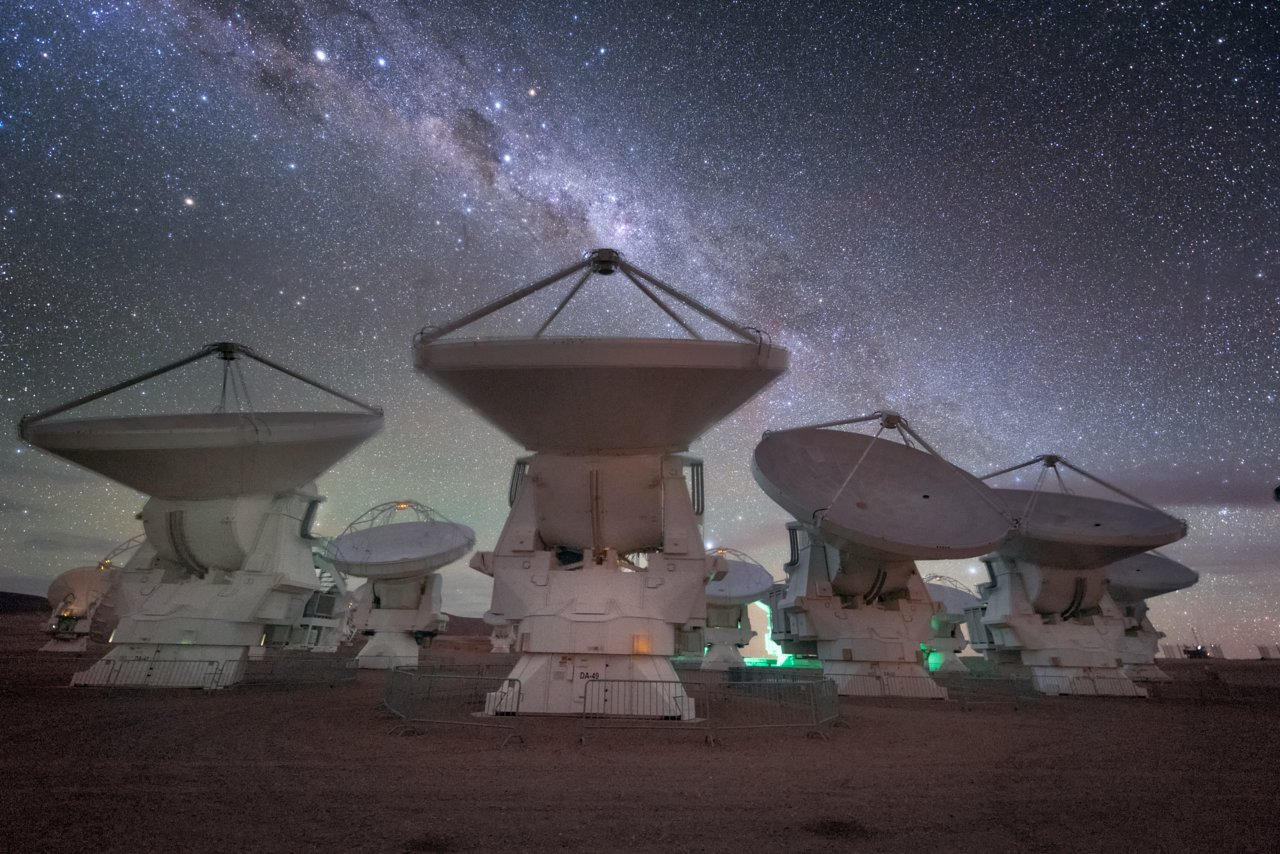
\includegraphics[width=0.70\textwidth]{Pictures/beletsky_alma_15-cc2.jpg}
\caption{Beletsky alma. https://www.eso.org/public/images/beletsky alma 15-cc2/}    
    \label{TELE}
\end{figure}

%\subsubsection{Forma canónica.}
\begin{exercise}
\item
Encuentre la forma canónica de la siguiente forma cuadrática:
$\mathbf{Q}(\vec{x})= x^2_2-3x^2_3 + 2x_1x_2 + x_1x_3$
\end{exercise}
\begin{exercise}
\item
Para la elipse $5x^2_1+5x^2_2 - 4x_1x_2 =48$, encuentre un cambio de variables por medio de calcular sus valores y vectores propios
unitarios tal que se elimine el producto cruzado de la ecuación.
\end{exercise}

\bigskip

%\subsubsection{Cónicas y su clasificación}

\vspace{0.25cm}
\begin{exercise}
\item
Especifique a que cónica corresponden las siguientes ecuaciones y especifique su centro.

\bigskip



a) $ (x-x_0)^2 + (y-y_0)^2=r^2$

b) $ (x-2)^2 - (y-3)^2=1$

c) $ x^2 +y^2 + 4x=1$
\end{exercise}

\newpage

\begin{exercise}
\item
Siendo la ecuación de una cónica:
$Ax^2+2Bxy+Cy^2+2Dx +2Ey+F=0$
Encuentre su forma matricial. Ayuda: Expresandola de la siguiente forma el elemento $a_{11}$ sería $F$, ¿cómo estarían relacionados los otros elementos de la matriz con la ecuación de la cónica?
  
  \begin{equation*}
\left(\begin{array}{ccc} 1 & x & y 
\end{array}
 \right) \left(\begin{array}{ccc} a_{11} &a_{12}  & a_{13}  \\a_{21} & a_{22} & a_{23} \\a_{31}  & a_{32} & a_{33}
\end{array}
 \right)  \left(\begin{array}{c} 1 \\x  \\y
\end{array}
 \right) =0\
\end{equation*}
Datos extras: Piense que las cónicas describen las órbitas. Ejemplo de órbitas elípticas pueden ser el  asteroide numerado 433 conocido con el nombre de Eros, en la página de  NEODyS (objetos cercanos al planeta Tierra) podrá encontrar muchos más.
Como ejemplo de órbita hiperbólica podría ser el  cometa C/2002 E2 Snyder-Murakami, y como ejemplo de órbita parábolica (excentricidad= 1) la del cometa C/2002 B2 LINEAR.

\bigskip

\end{exercise}
\begin{exercise}
\item
Usando la matriz del ejercicio anterior encuentre la forma de sus invariantes y especifique
de que tipo de cónica estamos hablando si $B^2-4AC=0$
\end{exercise}
\begin{exercise}
\item
Responda como estan los ejes de las cónicas con respecto a los ejes coordenados según:

a) $ B=0$

b) $ B\neq0$
\end{exercise}

\newpage

\begin{exercise}
\item
¿$\mathbf{Q}(\vec{x})= 3x^2_1+2x^2_2 + x^2_3 + 4x_1x_2 + 4x_2x_3$ es definida positiva?
\end{exercise}



 \subsection{ Autoevaluación}
 \label{Auto5}
 \bigskip



\subsubsection{Verdadero o Falso.}


 \bigskip
 
Dada una matriz simétrica:

\begin{enumerate}


 \item 
A es definida positiva si y solo si todos los valores propios de A son positivos.
\item
A es definida negativa si y solo si los valores propios van alternando entre positivos y negativos.
\item
A es indefinida si y solo si alguno de los valores propios es 0.
\item
Es posible clasificar A por medio de su determinante.
\item
Siempre exite un cambio ortogonal de la variable $\mathbf{x}=P\mathbf{y}$ tal que
$\mathbf{Q}(\mathbf{X})=\mathbf{x^t}A\mathbf{x}=\mathbf{y^t}D\mathbf{y}=\lambda_1x^2_1+\lambda_2x^2_2 + ... +\lambda_nx^2_n$
\end{enumerate}

